\documentclass[tikz,border=10pt]{standalone}
\begin{document}
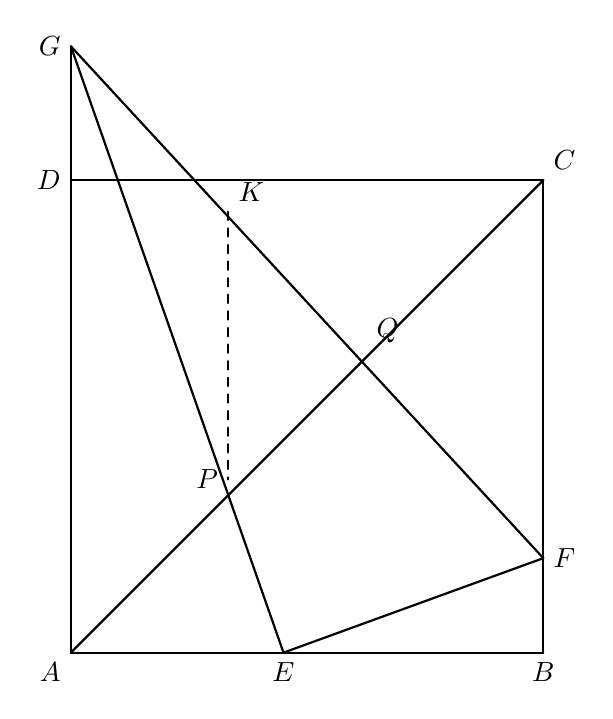
\begin{tikzpicture}[line cap=round,line join=round,thick]

% Coordinates
\coordinate (A) at (0,0);
\coordinate (B) at (6,0);
\coordinate (C) at (6,6);
\coordinate (D) at (0,6);
\coordinate (E) at (2.7,0);
\coordinate (F) at (6,1.2);
\coordinate (G) at (0,7.7);
\coordinate (K) at (2.0,5.6);
\coordinate (P) at (2.0,2.2);
\coordinate (Q) at (3.75,3.8);

% Outer shape
\draw (A) -- (B);
\draw (B) -- (C);
\draw (D) -- (C);
\draw (A) -- (G);

% Inner segments
\draw (G) -- (E);
\draw (G) -- (F);
\draw (A) -- (C);
\draw (E) -- (F);

% Dashed segment
\draw[dashed] (K) -- (P);

% Labels
\node[below left] at (A) {$A$};
\node[below] at (B) {$B$};
\node[above right] at (C) {$C$};
\node[left] at (D) {$D$};
\node[below] at (E) {$E$};
\node[right] at (F) {$F$};
\node[left] at (G) {$G$};
\node[above right] at (K) {$K$};
\node[left] at (P) {$P$};
\node[above right] at (Q) {$Q$};

\end{tikzpicture}
\end{document}
